% ============================================================================
% CHƯƠNG I: TỔNG QUAN VỀ HỆ THỐNG
% ============================================================================
\chapter{TỔNG QUAN VỀ HỆ THỐNG}

\section{Giới thiệu bài toán và mục tiêu hệ thống}

Trong bối cảnh số hóa và phát triển công nghệ thông tin, các thư viện truyền thống đang dần chuyển đổi sang mô hình thư viện điện tử (e-Library). Đối với các hệ thống thư viện có nhiều chi nhánh phân bố ở các vị trí địa lý khác nhau, việc quản lý tập trung và đồng bộ dữ liệu trở thành một thách thức lớn.

\subsection{Bài toán đặt ra}

Xây dựng một hệ thống quản lý thư viện điện tử phân tán với các yêu cầu:
\begin{itemize}
    \item Hỗ trợ nhiều chi nhánh hoạt động độc lập tại các vùng địa lý khác nhau
    \item Đảm bảo tính nhất quán dữ liệu giữa các chi nhánh
    \item Đảm bảo tính sẵn sàng cao (High Availability) khi có sự cố
    \item Hỗ trợ mở rộng quy mô theo nhu cầu
\end{itemize}

\subsection{Mục tiêu của đề tài}

\begin{enumerate}
    \item Thiết kế và cài đặt hệ thống thư viện phân tán sử dụng MongoDB Sharded Cluster
    \item Triển khai các kỹ thuật NoSQL nâng cao: Aggregation Pipeline, Map-Reduce, Zone Sharding
    \item Đảm bảo tính Fault Tolerance với MongoDB Replica Set
    \item Xây dựng giao diện web với Dashboard thống kê thời gian thực
\end{enumerate}

\section{Tổng quan về hệ thống e-Library}

\subsection{Mô hình hệ thống}

Hệ thống e-Library được thiết kế theo mô hình phân tán với 4 node:

\begin{table}[H]
\centering
\caption{Các node trong hệ thống e-Library}
\begin{tabular}{|c|l|l|l|}
\hline
\textbf{STT} & \textbf{Node} & \textbf{Database} & \textbf{Vai trò} \\
\hline
1 & Central Hub & Nhasach & Trung tâm quản lý \\
2 & Branch Hà Nội & NhasachHaNoi & Chi nhánh miền Bắc \\
3 & Branch Đà Nẵng & NhasachDaNang & Chi nhánh miền Trung \\
4 & Branch Hồ Chí Minh & NhasachHoChiMinh & Chi nhánh miền Nam \\
\hline
\end{tabular}
\end{table}

\subsection{Kiến trúc tổng quan}

\begin{figure}[H]
\centering
\begin{tikzpicture}[
    node distance=2cm,
    box/.style={rectangle, draw, minimum width=2.5cm, minimum height=1cm, align=center},
    cloud/.style={ellipse, draw, minimum width=3cm, minimum height=1.5cm, align=center},
]
    % Central Hub
    \node[box, fill=blue!20] (central) at (0,0) {Central Hub\\(Nhasach)};

    % Branches
    \node[box, fill=green!20] (hanoi) at (-4,-3) {Hà Nội\\(NhasachHaNoi)};
    \node[box, fill=yellow!20] (danang) at (0,-3) {Đà Nẵng\\(NhasachDaNang)};
    \node[box, fill=red!20] (hcm) at (4,-3) {Hồ Chí Minh\\(NhasachHoChiMinh)};

    % Connections
    \draw[<->] (central) -- (hanoi);
    \draw[<->] (central) -- (danang);
    \draw[<->] (central) -- (hcm);

    % MongoDB Cloud
    \node[cloud, fill=gray!10] (mongodb) at (0,3) {MongoDB\\Sharded Cluster};
    \draw[<->] (mongodb) -- (central);

\end{tikzpicture}
\caption{Kiến trúc tổng quan hệ thống e-Library phân tán}
\end{figure}

\section{Một số khái niệm và nghiệp vụ liên quan}

\subsection{Khái niệm về các đối tượng}

\begin{enumerate}
    \item \textbf{Quản trị viên hệ thống (System Admin)}: Quản lý toàn bộ hệ thống, cấu hình MongoDB, giám sát hoạt động của các node.

    \item \textbf{Quản trị viên cơ sở (Branch Admin)}: Quản lý sách, người dùng và giao dịch tại chi nhánh được phân công.

    \item \textbf{Nhân viên thư viện (Staff)}: Hỗ trợ người dùng mượn/trả sách, xử lý các yêu cầu tại quầy.

    \item \textbf{Khách hàng (Customer)}: Người dùng đăng ký tài khoản, tìm kiếm sách, mượn/trả sách online.
\end{enumerate}

\subsection{Các quy trình nghiệp vụ}

\begin{enumerate}
    \item \textbf{Đăng ký tài khoản}: Khách hàng đăng ký → Xác thực email → Kích hoạt tài khoản

    \item \textbf{Đăng nhập}: Nhập username/password → Xác thực JWT → Phân quyền truy cập

    \item \textbf{Tìm kiếm sách}: Nhập từ khóa → Full-text Search → Hiển thị kết quả với phân trang

    \item \textbf{Mượn sách}: Chọn sách → Thêm vào giỏ → Xác nhận đơn mượn → Thanh toán

    \item \textbf{Trả sách}: Nhân viên xác nhận → Cập nhật trạng thái → Tính phí trễ hạn (nếu có)

    \item \textbf{Đồng bộ dữ liệu}: Dữ liệu từ chi nhánh → API sync → Central Hub → Cập nhật dashboard

    \item \textbf{Thống kê báo cáo}: Aggregation Pipeline → Xử lý dữ liệu → Chart.js → Dashboard
\end{enumerate}

\section{Một số công nghệ được áp dụng}

\subsection{PHP 8.x và MongoDB Driver}

PHP (Hypertext Preprocessor) là ngôn ngữ lập trình kịch bản phía server, được sử dụng rộng rãi trong phát triển ứng dụng web. Trong đề tài này, nhóm sử dụng PHP 8.x kết hợp với thư viện \texttt{mongodb/mongodb} để xây dựng tầng API và giao diện web.

\textbf{Lý do lựa chọn PHP:}
\begin{itemize}
    \item Tương thích tốt với các máy chủ web thông dụng (Apache, Nginx)
    \item Thư viện \texttt{mongodb/mongodb} v2.1 hỗ trợ đầy đủ CRUD, Aggregation Pipeline
    \item Hỗ trợ BSON types cho làm việc với MongoDB
    \item Dễ triển khai mô hình MVC cho hệ thống phân tán
    \item Tích hợp tốt với JWT cho xác thực API
\end{itemize}

\textbf{Cài đặt MongoDB Driver cho PHP:}
\begin{lstlisting}[language=bash, caption=Cài đặt MongoDB Extension và Library]
# Cài đặt MongoDB PHP Extension
pecl install mongodb

# Cài đặt MongoDB PHP Library
composer require mongodb/mongodb:^2.1
\end{lstlisting}

\subsection{MongoDB và MongoDB Compass}

MongoDB là hệ quản trị cơ sở dữ liệu NoSQL hướng tài liệu (document-oriented), lưu trữ dữ liệu dưới dạng BSON (Binary JSON). MongoDB phiên bản 8.0.16 được sử dụng trong đề tài.

\textbf{Các tính năng MongoDB được sử dụng:}
\begin{itemize}
    \item \textbf{Replica Set}: Nhân bản dữ liệu giữa 3 node để đảm bảo High Availability
    \item \textbf{Sharding}: Phân mảnh dữ liệu theo vùng địa lý (Zone Sharding)
    \item \textbf{Aggregation Pipeline}: Xử lý và phân tích dữ liệu phức tạp
    \item \textbf{Map-Reduce}: Tính toán phân tán trên tập dữ liệu lớn
    \item \textbf{Text Search}: Tìm kiếm toàn văn với TEXT index
\end{itemize}

MongoDB Compass là công cụ GUI chính thức, hỗ trợ:
\begin{itemize}
    \item Trực quan hóa dữ liệu và cấu trúc schema
    \item Thực thi và tối ưu hóa Aggregation Pipeline
    \item Giám sát trạng thái Replica Set và Sharded Cluster
    \item Phân tích Explain Plan để tối ưu query
\end{itemize}

\subsection{Docker và Docker Compose}

Docker là nền tảng container hóa cho phép đóng gói ứng dụng cùng dependencies. Docker Compose cho phép định nghĩa multi-container applications trong một file YAML.

\textbf{Vai trò trong đề tài:}
\begin{itemize}
    \item Khởi tạo đồng thời 7 container MongoDB (3 config servers, 3 shard servers, 1 mongos)
    \item Giả lập mạng nội bộ cho giao tiếp giữa các node
    \item Dễ dàng tái lập kịch bản Failover
    \item Đảm bảo môi trường nhất quán giữa development và production
\end{itemize}

\subsection{Chart.js}

Chart.js là thư viện JavaScript mã nguồn mở để vẽ biểu đồ trên web. Phiên bản 4.4 được sử dụng cho Dashboard.

\textbf{Các loại biểu đồ được sử dụng:}
\begin{itemize}
    \item Bar Chart: Thống kê số lượng sách theo chi nhánh
    \item Pie Chart: Phân bố người dùng theo vai trò
    \item Line Chart: Xu hướng mượn sách theo thời gian
    \item Doughnut Chart: Tỷ lệ trạng thái đơn hàng
\end{itemize}

\subsection{JWT (JSON Web Token)}

JWT là chuẩn mở (RFC 7519) định nghĩa cách thức an toàn để truyền thông tin giữa các bên dưới dạng JSON object. Thư viện \texttt{firebase/php-jwt} được sử dụng cho xác thực API.

\textbf{Cấu trúc JWT:}
\begin{itemize}
    \item \textbf{Header}: Loại token và thuật toán mã hóa (HS256)
    \item \textbf{Payload}: Thông tin người dùng (user\_id, username, role, exp)
    \item \textbf{Signature}: Chữ ký số để xác thực tính toàn vẹn
\end{itemize}

% ============================================================================
% CHƯƠNG II: PHÂN TÍCH VÀ THIẾT KẾ HỆ THỐNG
% ============================================================================
\chapter{PHÂN TÍCH VÀ THIẾT KẾ HỆ THỐNG}

\section{Xác định các yêu cầu}

\subsection{Yêu cầu phi chức năng}

\begin{enumerate}
    \item \textbf{Tính sẵn sàng cao (High Availability)}: Hệ thống phải hoạt động liên tục 24/7, khả năng chịu lỗi khi 1/3 số node gặp sự cố.

    \item \textbf{Hiệu năng}: Thời gian phản hồi trung bình dưới 3ms cho các truy vấn cơ bản.

    \item \textbf{Khả năng mở rộng}: Hỗ trợ horizontal scaling, thêm node mới không cần downtime.

    \item \textbf{Bảo mật}: Xác thực JWT, mã hóa mật khẩu bcrypt, phân quyền RBAC.

    \item \textbf{Nhất quán dữ liệu}: Eventual consistency với replication lag dưới 500ms.
\end{enumerate}

\subsection{Yêu cầu chức năng}

\begin{table}[H]
\centering
\caption{Danh sách yêu cầu chức năng}
\begin{tabular}{|c|l|l|}
\hline
\textbf{STT} & \textbf{Chức năng} & \textbf{Mô tả} \\
\hline
1 & Đăng ký/Đăng nhập & Quản lý tài khoản người dùng \\
2 & Quản lý sách & CRUD sách, tìm kiếm, lọc \\
3 & Quản lý người dùng & CRUD người dùng, phân quyền \\
4 & Giỏ hàng & Thêm/xóa sách, tính tổng tiền \\
5 & Đặt mượn sách & Tạo đơn mượn, thanh toán \\
6 & Lịch sử mượn sách & Xem đơn đã mượn, trạng thái \\
7 & Dashboard thống kê & Biểu đồ Chart.js, số liệu realtime \\
8 & Đồng bộ dữ liệu & Sync giữa central và branches \\
\hline
\end{tabular}
\end{table}

\section{Ca sử dụng - Use Case}

\subsection{Danh sách các tác nhân}

\begin{table}[H]
\centering
\caption{Danh sách tác nhân trong hệ thống}
\begin{tabular}{|c|l|l|}
\hline
\textbf{STT} & \textbf{Tác nhân} & \textbf{Mô tả} \\
\hline
1 & Admin & Quản trị viên hệ thống, toàn quyền \\
2 & Customer & Khách hàng, mượn/trả sách \\
3 & System & Hệ thống tự động (sync, backup) \\
\hline
\end{tabular}
\end{table}

\subsection{Biểu đồ Use Case tổng quát}

\begin{figure}[H]
\centering
\begin{tikzpicture}[
    actor/.style={circle, draw, minimum size=0.8cm},
    usecase/.style={ellipse, draw, minimum width=2.5cm, minimum height=1cm, align=center, font=\small},
    node distance=1.5cm
]
    % Actors
    \node[actor] (admin) at (-5,0) {};
    \node[below=0.1cm of admin] {Admin};

    \node[actor] (customer) at (-5,-4) {};
    \node[below=0.1cm of customer] {Customer};

    % System boundary
    \draw[dashed] (-2.5,-6) rectangle (4,2);
    \node at (0.75,1.5) {e-Library System};

    % Use cases
    \node[usecase] (login) at (0,0.5) {Đăng nhập};
    \node[usecase] (manage_books) at (0,-0.8) {Quản lý sách};
    \node[usecase] (manage_users) at (0,-2.1) {Quản lý users};
    \node[usecase] (dashboard) at (0,-3.4) {Dashboard};
    \node[usecase] (browse) at (2.5,-0.8) {Xem sách};
    \node[usecase] (cart) at (2.5,-2.1) {Giỏ hàng};
    \node[usecase] (order) at (2.5,-3.4) {Đặt mượn};
    \node[usecase] (history) at (2.5,-4.7) {Lịch sử};

    % Connections - Admin
    \draw (admin) -- (login);
    \draw (admin) -- (manage_books);
    \draw (admin) -- (manage_users);
    \draw (admin) -- (dashboard);

    % Connections - Customer
    \draw (customer) -- (login);
    \draw (customer) -- (browse);
    \draw (customer) -- (cart);
    \draw (customer) -- (order);
    \draw (customer) -- (history);

\end{tikzpicture}
\caption{Biểu đồ Use Case tổng quát}
\end{figure}

\section{Mô hình cấu trúc}

\subsection{Danh sách các lớp đối tượng}

Từ phân tích yêu cầu, hệ thống bao gồm các lớp đối tượng chính:

\begin{enumerate}
    \item \textbf{User}: Quản lý thông tin người dùng
    \begin{itemize}
        \item Thuộc tính: \_id, username, password, fullname, email, role, balance, location, status
        \item Phương thức: login(), logout(), register(), updateProfile()
    \end{itemize}

    \item \textbf{Book}: Quản lý thông tin sách
    \begin{itemize}
        \item Thuộc tính: \_id, bookCode, bookName, bookGroup, author, quantity, pricePerDay, borrowCount, location
        \item Phương thức: create(), update(), delete(), search(), getByLocation()
    \end{itemize}

    \item \textbf{Cart}: Quản lý giỏ hàng
    \begin{itemize}
        \item Thuộc tính: \_id, user\_id, items[], total\_quantity, total\_amount
        \item Phương thức: addItem(), removeItem(), clear(), checkout()
    \end{itemize}

    \item \textbf{Order}: Quản lý đơn mượn sách
    \begin{itemize}
        \item Thuộc tính: \_id, user\_id, items[], status, borrow\_date, return\_date, total\_amount
        \item Phương thức: create(), updateStatus(), calculateFee()
    \end{itemize}

    \item \textbf{Activity}: Ghi log hoạt động
    \begin{itemize}
        \item Thuộc tính: \_id, action, user\_id, details, timestamp, ip\_address
        \item Phương thức: log(), getByUser(), getByAction()
    \end{itemize}
\end{enumerate}

\subsection{Biểu đồ lớp}

\begin{figure}[H]
\centering
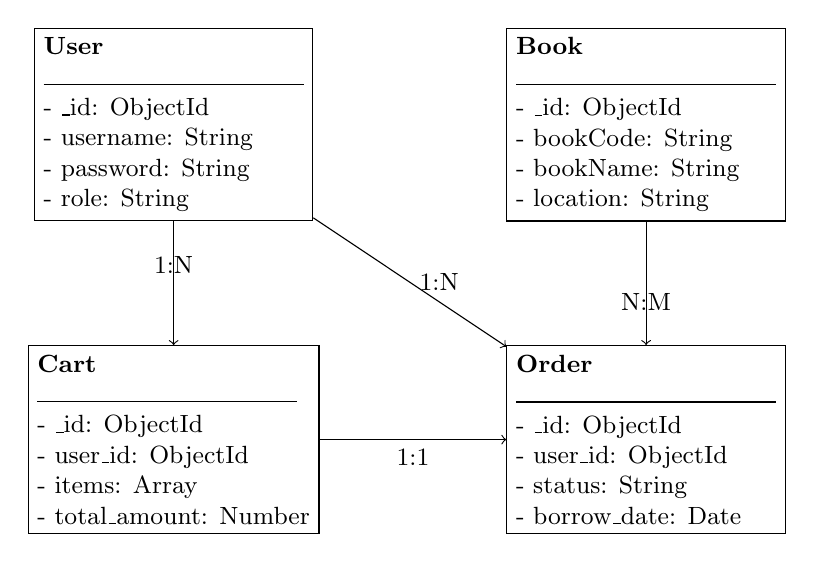
\begin{tikzpicture}[
    class/.style={rectangle, draw, minimum width=3.5cm, minimum height=2cm, align=left, font=\small},
    node distance=3.5cm
]
    % Classes
    \node[class] (user) at (0,0) {
        \textbf{User}\\
        \rule{3.3cm}{0.4pt}\\
        - \_id: ObjectId\\
        - username: String\\
        - password: String\\
        - role: String
    };

    \node[class] (book) at (6,0) {
        \textbf{Book}\\
        \rule{3.3cm}{0.4pt}\\
        - \_id: ObjectId\\
        - bookCode: String\\
        - bookName: String\\
        - location: String
    };

    \node[class] (cart) at (0,-4) {
        \textbf{Cart}\\
        \rule{3.3cm}{0.4pt}\\
        - \_id: ObjectId\\
        - user\_id: ObjectId\\
        - items: Array\\
        - total\_amount: Number
    };

    \node[class] (order) at (6,-4) {
        \textbf{Order}\\
        \rule{3.3cm}{0.4pt}\\
        - \_id: ObjectId\\
        - user\_id: ObjectId\\
        - status: String\\
        - borrow\_date: Date
    };

    % Relationships
    \draw[->] (user) -- node[above, font=\small] {1:N} (cart);
    \draw[->] (user) -- node[right, font=\small] {1:N} (order);
    \draw[->] (book) -- node[below, font=\small] {N:M} (order);
    \draw[->] (cart) -- node[below, font=\small] {1:1} (order);

\end{tikzpicture}
\caption{Biểu đồ lớp hệ thống e-Library}
\end{figure}

\section{Thiết kế CSDL}

\subsection{Xác định các collection}

\begin{table}[H]
\centering
\caption{Danh sách collection trong MongoDB}
\begin{tabular}{|c|l|l|l|}
\hline
\textbf{STT} & \textbf{Collection} & \textbf{Mô tả} & \textbf{Số documents} \\
\hline
1 & users & Thông tin người dùng & 38 \\
2 & books & Danh mục sách & 909 \\
3 & carts & Giỏ hàng & Dynamic \\
4 & orders & Đơn mượn sách & 46 \\
5 & activities & Log hoạt động & Dynamic \\
6 & customers & Khách hàng tổng hợp (Central) & 33 \\
\hline
\end{tabular}
\end{table}

\subsection{Thiết kế bảng dữ liệu vật lý}

\textbf{Collection users:}
\begin{lstlisting}[language=json, caption=Schema collection users]
{
    "_id": ObjectId,
    "username": String (unique),
    "password": String (bcrypt hash),
    "fullname": String,
    "email": String,
    "role": "admin" | "customer",
    "balance": Number,
    "location": String,
    "status": "active" | "inactive",
    "created_at": ISODate,
    "updated_at": ISODate
}
\end{lstlisting}

\textbf{Collection books:}
\begin{lstlisting}[language=json, caption=Schema collection books]
{
    "_id": ObjectId,
    "bookCode": String (unique),
    "bookName": String,
    "bookGroup": String,
    "author": String,
    "description": String,
    "quantity": Number,
    "pricePerDay": Number,
    "borrowCount": Number,
    "location": "Ha Noi" | "Da Nang" | "Ho Chi Minh",
    "status": "active" | "deleted"
}
\end{lstlisting}

\textbf{Collection orders:}
\begin{lstlisting}[language=json, caption=Schema collection orders]
{
    "_id": ObjectId,
    "user_id": ObjectId,
    "username": String,
    "items": [
        {
            "bookCode": String,
            "bookName": String,
            "quantity": Number,
            "pricePerDay": Number,
            "days": Number,
            "subtotal": Number
        }
    ],
    "total_quantity": Number,
    "total_amount": Number,
    "status": "pending" | "paid" | "success" | "returned",
    "borrow_date": ISODate,
    "return_date": ISODate,
    "created_at": ISODate
}
\end{lstlisting}

\subsection{Thiết kế mô hình phân tán}

\begin{figure}[H]
\centering
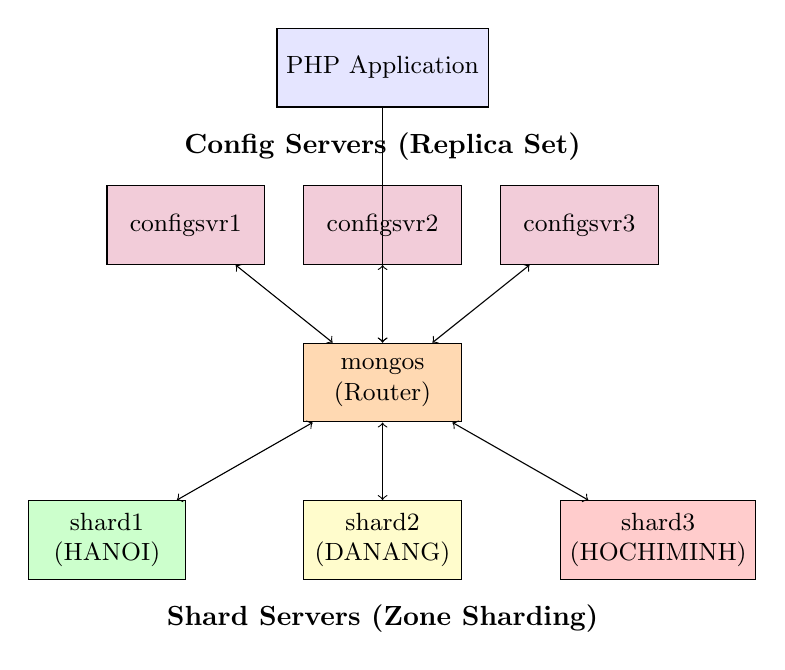
\begin{tikzpicture}[
    container/.style={rectangle, draw, minimum width=2cm, minimum height=1cm, align=center, font=\small},
    zone/.style={rectangle, draw, dashed, minimum width=3cm, minimum height=4cm, align=center},
    node distance=1cm
]
    % Config Servers
    \node[container, fill=purple!20] (config1) at (0,3) {configsvr1};
    \node[container, fill=purple!20] (config2) at (2.5,3) {configsvr2};
    \node[container, fill=purple!20] (config3) at (5,3) {configsvr3};
    \node at (2.5,4) {\textbf{Config Servers (Replica Set)}};

    % Mongos
    \node[container, fill=orange!30] (mongos) at (2.5,1) {mongos\\(Router)};

    % Shard Servers
    \node[container, fill=green!20] (shard1) at (-1,-1) {shard1\\(HANOI)};
    \node[container, fill=yellow!20] (shard2) at (2.5,-1) {shard2\\(DANANG)};
    \node[container, fill=red!20] (shard3) at (6,-1) {shard3\\(HOCHIMINH)};
    \node at (2.5,-2) {\textbf{Shard Servers (Zone Sharding)}};

    % Connections
    \draw[<->] (mongos) -- (config1);
    \draw[<->] (mongos) -- (config2);
    \draw[<->] (mongos) -- (config3);
    \draw[<->] (mongos) -- (shard1);
    \draw[<->] (mongos) -- (shard2);
    \draw[<->] (mongos) -- (shard3);

    % Client
    \node[container, fill=blue!10] (client) at (2.5,5) {PHP Application};
    \draw[->] (client) -- (mongos);

\end{tikzpicture}
\caption{Kiến trúc MongoDB Sharded Cluster}
\end{figure}

\subsection{Thiết kế tìm kiếm và tối ưu truy vấn}

Hệ thống sử dụng các index để tối ưu hiệu năng:

\begin{table}[H]
\centering
\caption{Danh sách Index trong collection books}
\begin{tabular}{|l|l|l|}
\hline
\textbf{Index Name} & \textbf{Fields} & \textbf{Mục đích} \\
\hline
bookCode\_1 & \{bookCode: 1\} & Unique index, point lookup \\
location\_1\_bookName\_1 & \{location: 1, bookName: 1\} & Shard-aware queries \\
bookName\_text\_bookGroup\_text & TEXT index & Full-text search \\
borrowCount\_-1 & \{borrowCount: -1\} & Sắp xếp sách phổ biến \\
\hline
\end{tabular}
\end{table}

\textbf{Full-text Search:}
\begin{lstlisting}[language=PHP, caption=Tìm kiếm toàn văn trong PHP]
<?php
// Tạo TEXT index
$db->books->createIndex([
    'bookName' => 'text',
    'bookGroup' => 'text',
    'author' => 'text',
    'description' => 'text'
], ['name' => 'idx_text_search']);

// Thực hiện tìm kiếm
$results = $db->books->find([
    '$text' => ['$search' => $keyword]
], [
    'projection' => ['score' => ['$meta' => 'textScore']],
    'sort' => ['score' => ['$meta' => 'textScore']]
]);
\end{lstlisting}

\section{Thiết kế giao diện}

Giao diện hệ thống được thiết kế theo nguyên tắc:
\begin{itemize}
    \item Responsive design: Tương thích đa thiết bị
    \item Bootstrap 5: Framework CSS hiện đại
    \item Chart.js: Biểu đồ tương tác
    \item AJAX: Cập nhật dữ liệu không tải lại trang
\end{itemize}

Các giao diện chính sẽ được trình bày chi tiết trong Chương III - Cài đặt và Đánh giá.
